\section{Fatigue}
\begin{multicols} 2
	
	While dealing fatigue important is firstly to define the maximum $\sigma_{max}$, the minimum $\sigma_{min}$ stresses on the section of interest, but also the mean value $\sigma_m$ and the amplitude $\sigma_a$ due to the oscillating load:
	\[ \sigma_m = \frac{\sigma_{max} + \sigma_{min}}{2} \qquad \sigma_a = \frac{\sigma_{max} - \sigma_{min}}{2} \]
	
	Related to the component it's important to define the \textbf{notch fatigue factor} $K_f$ that depends on the parameter $q$ and the stress concentration factor $K_t$; both value are usually tabulated in dependence of the geometrical property of the section and it allows to compute the notch fatigue factor which is equal to
	\begin{equation}
		K_f = 1 + q \big(K_t-1\big)
	\end{equation}
	If $q$ cannot be derived from the diagram (even with extrapolation), choosing $q=1$ is always a conservative decision. \vspace{3mm}
	
	The next stage is to calculate all the coefficients that allows to compute the allowable tension $\sigma_{all}$; the first parameter is $C_s$ that's related to the surface finishes and depends on the ultimate tensile strength UTS $\sigma_r$ (in $MPa$) and two coefficients $a,b$ usually tabulated (table \ref{tab:surfacefinish}):
	\begin{equation} \label{eq:surfacefinish}
		C_s = a \,\sigma_r ^b
	\end{equation}
	Next we need to define the coefficient related to the dimension $d$ of the section; in order to do so it's important to determine a relation that allows to compute a equivalent diameter $d_{ed}$	for a generic section: this can be done by determining the diameter of a circle that has the same area as the section $d_{eq} = \sqrt{\frac 4\pi A}$. Done this it's possible to compute the dimension coefficient $C_d$:
	\begin{equation}
		C_d = \begin{cases}
			1 & d< 8mm \\
			1.189 d^{-0.097} \quad & 8mm < d < 250mm \\
			0.6 & d > 250mm
		\end{cases}
	\end{equation}
	The last coefficient $C_l$ is associated to the load and depends only on the way the material is stressed:
	\begin{equation}
		C_{l} = \begin{cases}
			1 & \textrm{bending, torsion} \\
			0.6 \quad & \textrm{axial loading}
		\end{cases}
	\end{equation}
	With all those factor computed we can calculate the allowable stress $\sigma_{all}$ depending also the fatigue limit stress $\sigma_{lim}$ and the safe factor $\phi$:
	\begin{equation}
		\sigma_{all} = \frac{C_sC_dC_l}{\phi} \sigma_{lim}
	\end{equation} \vspace{3mm}

	At this stage we have all the components to verify (or dimension, depending on the process) the component; the $SN$ curves are described by test where the mean value of the stress is zero ($\sigma_m = 0$), but general loads can have various combination of $\sigma_m,\sigma_a$: in order to do so we use the isocritical stress method, that with a linear relation permit to calculate the equivalent amplitude $\sigma_a^*$ as
	\begin{equation}
		\sigma_a^* = \sigma_y \frac{\sigma_a}{\sigma_y - \sigma_m}
	\end{equation}
	In order to include the possible plasticisation due to the non-zero mean stress, it's possible to use the following criteria that modify the nominal mean stress $\sigma_{m,nom}$ depending from the stress concentration factor $K_t$:
	\[ \sigma_m = \begin{cases}
		\sigma_{m,nom} & K_t \sigma_{max} > \sigma_y \\
		K_f\sigma_{m,nom} \quad & K_t \sigma_{max} \leq \sigma_y \\
	\end{cases} \]
	\begin{center}
		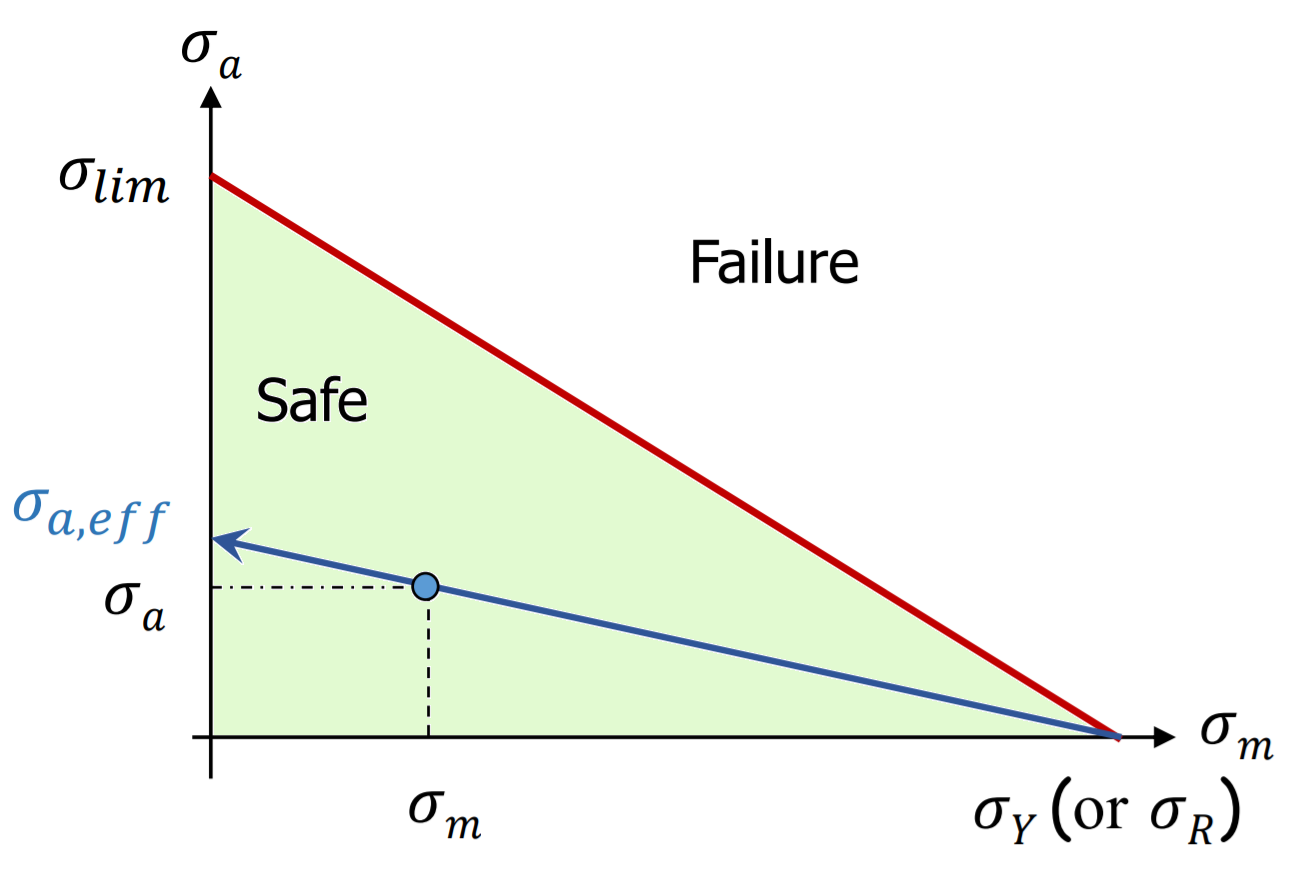
\includegraphics[width=5.5cm]{isocritical-fatigue}
	\end{center}
\end{multicols}
	
	\begin{SCtable}[1][bht]
		\centering
		\begin{tabular}{r || c | c}
			\textbf{surface finish} & factor $a$ & exponent $b$ \\ \hline
			ground & 1.58 & -0.085 \\
			machined or cold-drawn & 4.51 & -0.265 \\
			hot-rolled & 57.7 & -0.718 \\
			as-forged & 272 & -0.995
		\end{tabular}
		\caption{coefficients to determine the surface effect coefficient (equation \ref{eq:surfacefinish}).}
		\label{tab:surfacefinish}
	\end{SCtable}

\begin{multicols} 2
\subsection*{SN diagrams}
	The simplest function that's use to relate the number of cycle to failure $N_f$ with the alternate stress $\sigma_a$ is the Basquin law
	\begin{equation}
		\sigma_a = C N_f ^{-\frac 1 k}
	\end{equation}
	\begin{center}
		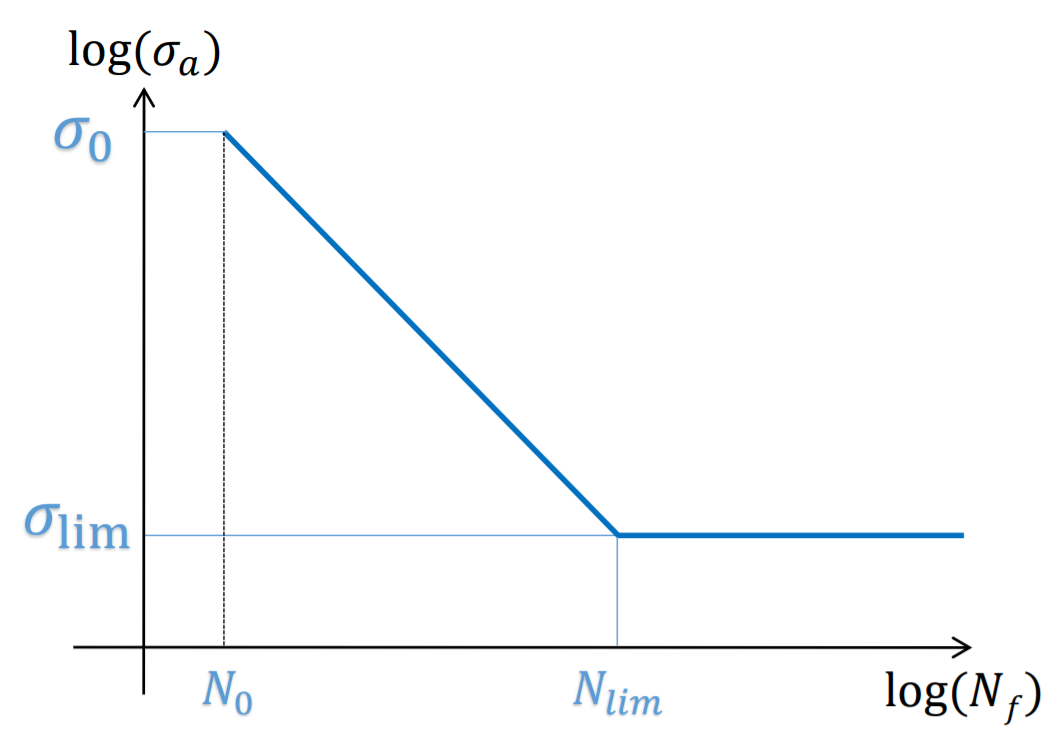
\includegraphics[width=5cm]{SNbasquin}
	\end{center}
	
	This relation is made to fit, as seen in the shown diagram, the linear logarithmic relation between the stress and the cycles to failure; in particular known the limit tension $\sigma_{lim}$ and the related cycle $N_{lim}$ and another experimental point $\sigma_0, N_0$, it's possible to compute the coefficient $C$ and $1/k$ of the law:
	\[ \frac 1 k = \frac{-\log \left( \frac{\sigma_{lim}}{\sigma_0} \right) }{\log \left( \frac{N_{lim}}{N_0} \right)}  \qquad C = \frac{\sigma_{lim}}{N_{lim}^{-\frac 1 k}} \]
	In general the fatigue limit (for steels) can be computed as
	\[ \sigma_{lim} = \begin{cases}
		0.5 \sigma_r \qquad & \sigma_r \leq 1400MPa \\
		700 MPa & \sigma_r>1400MPa
	\end{cases}  \]

\subsection*{Damage}
	In order to take into account the damage $D$ due to fatigue it's possible to use a linear operation (that allow to take into account multi-variable load) defined as
	\[ D = \sum_i \frac{n_i}{N_{f,i}} \leq 1 \]
	where $n_i$ is the number of cycles at certain combination of cyclic stress with mean value $\sigma_{m,i}$ and amplitude $\sigma_{a,i}$ that determines a number of fatigue fracture cycles $N_{f,i}$. By using conventional method to compute $N_f$, if the component is subject to a stress less than $\sigma_{lim}$ than the damage should be zero, but in reality it's not: in this case we revise the SN diagram in order to take into account that factor by using not a straight line after $N_{lim}$, but one relation in the form
	\[ \sigma_a = C'N_f^{-\frac{1}{2k-1}} \]
	\begin{center}
		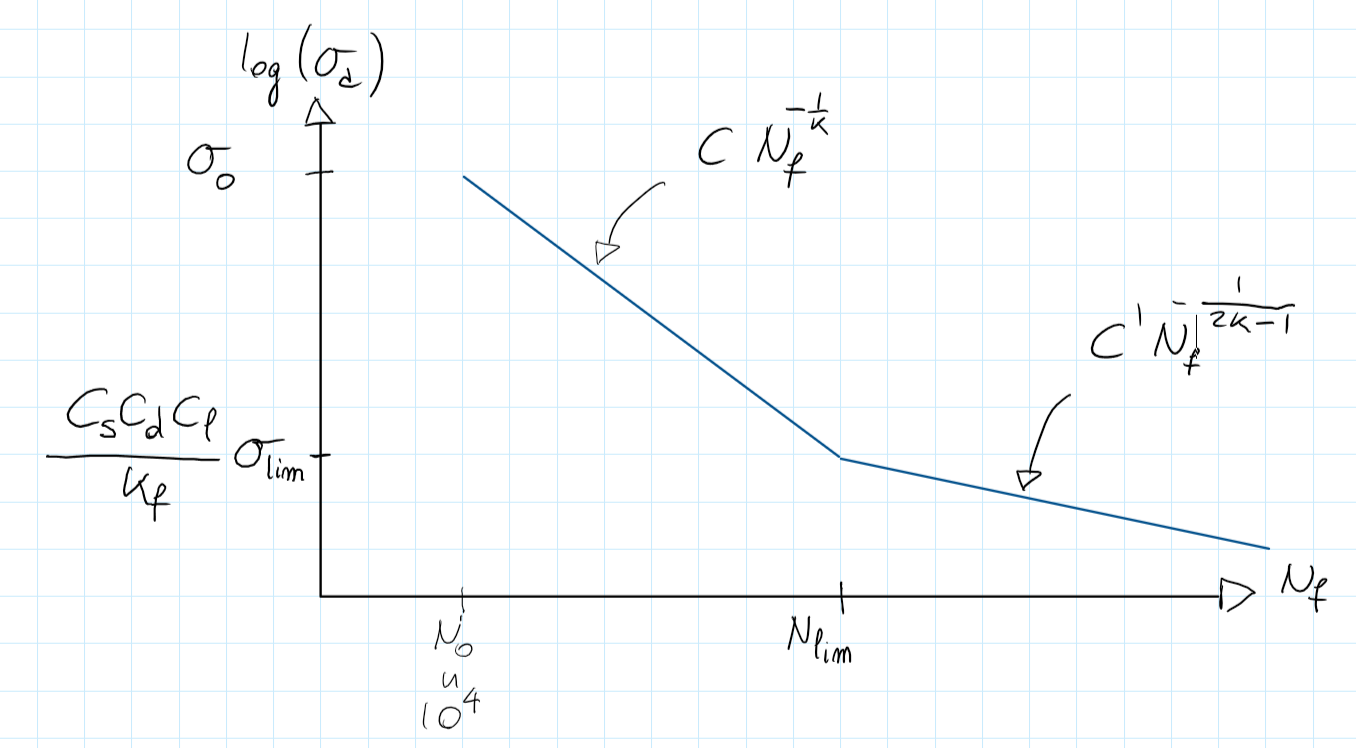
\includegraphics[width=6.5cm]{SNdamage}
	\end{center}
	Pay attention when doing so at including also the effect of the coefficients $C_s,C_d,C_l$ and $K_f$.



\end{multicols}






